% ICASSP-style draft prepared with the official reachable ICASSP paper kit.
\documentclass{article}
\usepackage{spconf,amsmath,amssymb,amsthm,graphicx,booktabs,multirow,cite,url}
\usepackage[colorlinks=true,urlcolor=blue]{hyperref}

\def\z{{\mathbf z}}
\def\x{{\mathbf x}}
\def\eps{{\boldsymbol \epsilon}}
\def\del{{\boldsymbol \delta}}
\newcommand{\Rcert}{R_{\mathrm{cert}}}
\newcommand{\punder}{\underline{p_A}}
\newcommand{\Smanifold}{\mathcal{S}}

\newtheorem{theorem}{Theorem}
\newtheorem{corollary}{Corollary}
\newtheorem{assumption}{Assumption}

\title{CertAV: Manifold-Aware Certified Robustness for\\ Audio-Visual Deepfake Detection}

\name{Palak Parmar$^{1*}$, Chintan Bhatt$^2$ and SantoshKumar Bharti$^1$}
\address{$^{1*}$Department of Computer Science and Engineering, School of Science\\
and Technology, Pandit Deendayal Energy University, Gandhinagar,\\
Gujarat, India.\\
$^2$School of Computing and Information Technology, University of\\
Wollongong, Australia.\\[0.5em]
$^*$Corresponding author(s). E-mail(s): \href{mailto:24rcp002@sot.pdpu.ac.in}{24rcp002@sot.pdpu.ac.in};\\
Contributing authors: \href{mailto:cbhatt@uow.edu.au}{cbhatt@uow.edu.au};\\
\href{mailto:santosh.bharti@sot.pdpu.ac.in}{santosh.bharti@sot.pdpu.ac.in};}

\begin{document}
\ninept
\maketitle

\begin{abstract}
Audio-visual deepfake detectors rely on frozen foundation representations, yet their robustness is typically evaluated only empirically. We introduce CertAV, a certification framework that applies randomized smoothing in the joint feature space of frozen DINOv2 and Whisper encoders. On FakeAVCeleb, CertAV reaches $92.5\%$ clean accuracy and $88.0\%$ certified accuracy at $\ell_2$ radius $1.0$, with less than $1\%$ abstention. We prove that, under a subspace-invariance property of the detector head, the smoothed classifier's certified radius depends only on the $d$-dimensional on-manifold component of the noise ($d\!\approx\!80 \ll D\!=\!768$), implying a robustness amplification factor of $\sqrt{D/d}$. Validating this across five encoder families, we confirm that a lower intrinsic-dimension ratio $d/D$ yields larger certified radii. Exploiting this geometry, we propose manifold-aware anisotropic smoothing that, at equalized noise budget, achieves a $3.4\times$ larger on-manifold certified radius ($7.63$ vs.\ $2.22$) with zero abstention. The same geometry explains an ablation finding: a no-noise baseline certifies within $1.9\%$ of the noise-trained model, indicating that certifiability is set primarily by representation geometry rather than by the training procedure.
\end{abstract}

\begin{keywords}
audio-visual deepfake detection, certified robustness, randomized smoothing, anisotropic smoothing, media forensics
\end{keywords}

\section{Introduction}
\label{sec:intro}

Audio-visual deepfake detection has moved from single-stream artifact recognition toward cross-modal reasoning: whether a face, voice, expression, and temporal speech pattern belong to the same event. Modern detectors increasingly build on frozen self-supervised encoders, and while they are accurate under clean evaluation, they can remain vulnerable to small adversarial feature shifts. For forensic use, a calibrated detector is useful; a detector with a per-sample robustness certificate is stronger.

Randomized smoothing converts a base classifier into a smoothed classifier whose prediction is provably unchanged within an $\ell_2$ ball around its input \cite{cohen2019certified}. Its common use is image-space classification, where the radius is measured in pixels. Audio-visual deepfake detection is less straightforward: videos are long, audio is continuous, and detectors typically consume frozen DINOv2 \cite{oquab2024dinov2} and Whisper \cite{radford2023whisper} features rather than raw input. CertAV therefore certifies the detector in this joint feature space. This is a deliberately scoped guarantee: it does not certify arbitrary waveform or pixel perturbations, but gives an exact robustness statement for the representation actually consumed by the detector.

The central observation is that feature-space smoothing gives large certified radii with little abstention, and that this is not primarily an effect of noise-augmented training. Instead, the frozen multimodal representation is low-dimensional relative to its ambient feature space, so isotropic Gaussian noise can move a sample substantially without crossing the decision boundary. We make this precise: under a subspace-invariance property of the detector head, the certified radius is governed only by the on-manifold noise, and the gap between an adversary's ambient budget and its on-manifold effect scales as $\sqrt{D/d}$. This explains the observed radii, predicts which encoders certify best, and motivates a smoothing distribution aligned to the manifold.

This paper makes four contributions.
(i) We define \emph{CertAV}, a feature-space randomized-smoothing pipeline for audio-visual deepfake detection under a joint $\ell_2$ threat model.
(ii) We prove a \emph{Certifiability Scaling} theorem and a \emph{Robustness Amplification} corollary that explain why frozen multimodal features certify well and give a principled encoder-selection criterion.
(iii) We validate the theory with an \emph{encoder-scaling study} across five visual/audio encoder families, confirming that lower $d/D$ yields larger certified radii.
(iv) We propose \emph{manifold-aware anisotropic smoothing}, which at equalized noise budget achieves a $3.4\times$ larger on-manifold certified radius with zero abstention.

\section{Related Work}
\label{sec:related}

\noindent\textbf{Audio-visual deepfake detection.}
Audio-visual detectors exploit inconsistencies invisible in either modality alone, from affective disagreement \cite{mittal2020emotions} and audio-visual dissonance \cite{chugh2020not} to self-supervised anomaly detection \cite{feng2023self}, joint learning \cite{yang2023avoid}, and local temporal inconsistency modeling \cite{astrid2025local}. Datasets such as FakeAVCeleb \cite{khalid2021fakeavceleb} and LAV-DF \cite{cai2022lavdf} provide multimodal settings. These works improve accuracy and localization, but their robustness claims are largely empirical.

\noindent\textbf{Certified robustness.}
Randomized smoothing certifies an $\ell_2$ ball by estimating the probability that a Gaussian-perturbed base classifier predicts the top class \cite{cohen2019certified,lecuyer2019certified,salman2019provably}. Yang et al.\ \cite{yang2020randomized} generalize this to arbitrary noise distributions, showing that non-isotropic smoothing yields ellipsoidal certified regions, and ANCER \cite{eiras2022ancer} optimizes per-sample anisotropic noise to maximize certified volume. MMCert \cite{wang2024mmcert} certifies multimodal models by randomized ablation of raw inputs. CertAV differs by certifying the frozen \emph{feature} space consumed by the detector, by giving a theoretical account of why this space certifies well, and by using a simple global PCA-aligned anisotropic distribution justified by that account rather than per-sample volume optimization.

\section{Method}
\label{sec:method}

\begin{figure}[t]
\centering
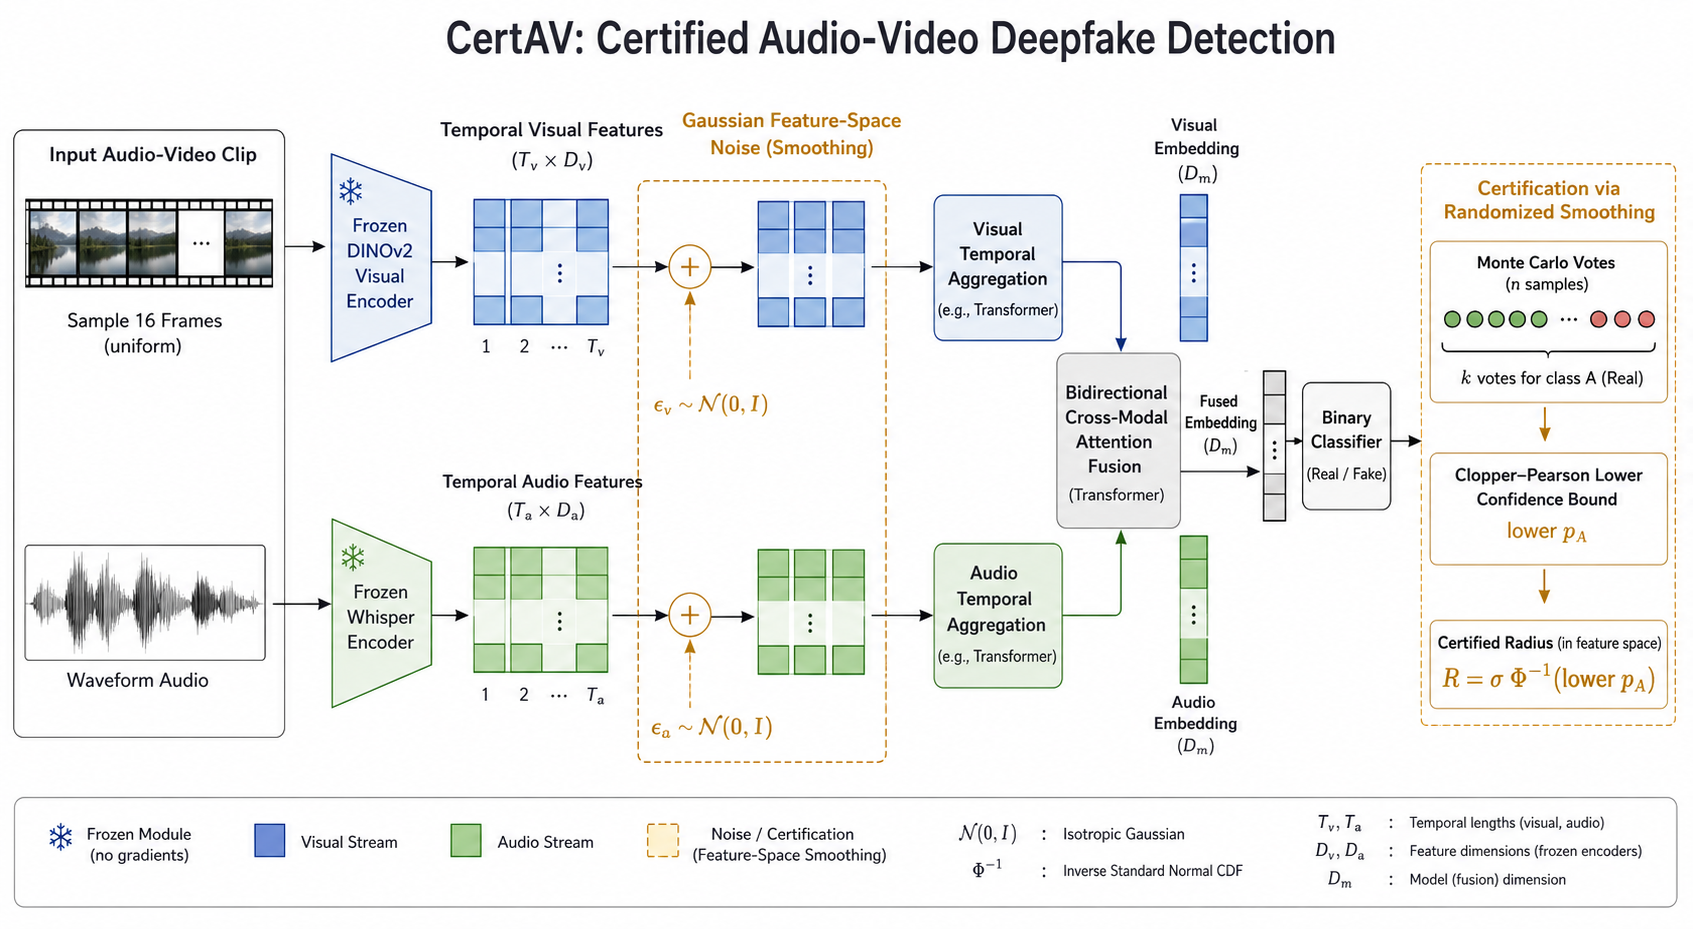
\includegraphics[width=\linewidth]{figures/certav_architecture.png}
\caption{CertAV pipeline. Frozen DINOv2 and Whisper encoders produce temporal visual and audio features, which are aggregated, fused by bidirectional cross-modal attention, and certified by randomized smoothing in joint feature space.}
\label{fig:architecture}
\vspace{-0.3cm}
\end{figure}

\subsection{Feature representation and detector}
\label{ssec:detector}

Given an audio-video clip $\x$, CertAV extracts visual and audio feature sequences $Z_v = E_v(\x_v)$ and $Z_a = E_a(\x_a)$, where $E_v$ is a frozen DINOv2-Small encoder (16 frames, $384$-d embeddings) and $E_a$ is a frozen Whisper-tiny encoder (16\,kHz audio up to $10$\,s, $384$-d temporal embeddings). The base detector $f_\theta$ projects each modality to a $256$-d temporal sequence (a transformer aggregator for video, temporal pooling for audio), applies a two-layer bidirectional cross-modal attention module, and averages segment logits before a binary real/fake decision. Features are cached and used as the input domain for training, attacks, and certification.

\subsection{Threat model and certification}
\label{ssec:threat}

Let $\z=(Z_v,Z_a)\in\mathbb{R}^D$ ($D=768$) denote the concatenated frozen representation. CertAV certifies robustness to joint feature perturbations $\del$ with $\|\del\|_2\le r$. This is the correct abstraction for frozen-encoder pipelines, where the detector never observes raw input: certifying the giant frozen encoders end-to-end is computationally intractable and yields vanishingly small radii, whereas the feature-space certificate is exact for any adversary acting on the representation the detector consumes. To connect the two spaces we additionally measure an empirical feature-to-input Lipschitz constant $L$ from input-space attacks and compose it with the feature certificate; on FakeAVCeleb $L\!\approx\!50$, mapping the on-manifold certificate to an approximate input-space radius of $\approx\!0.12$ at $\approx\!90.7\%$ composed certified accuracy. The smoothed classifier is
\begin{equation}
  g(\z)=\arg\max_c \Pr_{\eps\sim\mathcal{N}(0,\sigma^2 I)}\!\left(f_\theta(\z+\eps)=c\right).
\end{equation}
During training, Gaussian noise $\eps\sim\mathcal{N}(0,\sigma^2 I)$ is injected into the features and the model is fit with binary cross-entropy. Certification follows the two-stage Monte Carlo procedure of \cite{cohen2019certified}: $n_0=100$ samples select the candidate class, $n=1000$ samples estimate its probability, and a Clopper-Pearson lower bound $\punder$ ($\alpha=0.001$) gives the certified radius $\Rcert=\sigma\,\Phi^{-1}(\punder)$, abstaining if $\punder\le 0.5$.

\subsection{Manifold-aware anisotropic smoothing}
\label{ssec:aniso}

Let $\Smanifold$ be the $d$-dimensional subspace spanned by the top principal components of the training features (the $90\%$-variance threshold gives $d\!\approx\!80$). Anisotropic smoothing replaces isotropic $\mathcal{N}(0,\sigma^2 I)$ by $\mathcal{N}(0,\Sigma)$ with $\Sigma$ diagonal in the PCA basis. All strategies preserve the \emph{total} noise budget, $\mathrm{trace}(\Sigma)=D\sigma^2$, so improvements come from \emph{redistributing} noise, not adding it. We report two radii: the worst-case $\ell_2$ radius $R_{\ell_2}=\Phi^{-1}(\punder)\sqrt{\lambda_{\min}(\Sigma)}$ (largest inscribed sphere), and the on-manifold radius $R_{\Smanifold}=\Phi^{-1}(\punder)\sqrt{\bar\lambda_{\Smanifold}}$, where $\bar\lambda_{\Smanifold}$ is the mean variance over the top-$d$ directions in which the decision boundary lies.

\section{Theoretical Analysis}
\label{sec:theory}

Let $P_\Smanifold$ project onto $\Smanifold$ and $P_\perp=I-P_\Smanifold$ onto its complement.

\begin{assumption}[Subspace invariance]
\label{assm:subspace}
For all $\z\in\Smanifold$ and all $\del\in\mathbb{R}^D$, $f(\z+\del)=f(\z+P_\Smanifold\del)$: only the on-manifold component of a perturbation affects the classifier.
\end{assumption}

This is an idealization, justified because $f$ is trained on features drawn from $\Smanifold$ and receives no gradient from off-manifold directions; we validate it empirically below.

\begin{theorem}[Certifiability scaling]
\label{thm:scaling}
Under Assumption~\ref{assm:subspace}, for any $\z\in\Smanifold$ the top-class probability $p_A$ of the smoothed classifier with $\eps\sim\mathcal{N}(0,\sigma^2 I_D)$ depends on $\eps$ only through its projection $\eps_\Smanifold=P_\Smanifold\eps\sim\mathcal{N}(0,\sigma^2 I_d)$, and the certified radius is $\Rcert=\sigma\,\Phi^{-1}(p_A)$.
\end{theorem}

\noindent\emph{Proof sketch.} Decompose $\eps=\eps_\Smanifold+\eps_\perp$. Because $P_\Smanifold$ and $P_\perp$ are complementary orthogonal projections, $\eps_\Smanifold$ and $\eps_\perp$ are independent Gaussians. By Assumption~\ref{assm:subspace}, $f(\z+\eps)=f(\z+\eps_\Smanifold)$ for every $\eps_\perp$, so $p_A$ is determined by the $d$-dimensional variable $\eps_\Smanifold$; the radius then follows from \cite{cohen2019certified}.\hfill$\square$

\begin{corollary}[Robustness amplification]
\label{cor:amp}
For an adversary with budget $\|\del\|_2\le r$ and direction uniform on $\mathbb{S}^{D-1}$, $\mathbb{E}\,\|P_\Smanifold\del\|_2^2=(d/D)\,r^2$, so achieving on-manifold displacement $m$ requires $r\ge m\sqrt{D/d}$. The amplification factor is $\mathcal{A}=\sqrt{D/d}$; among encoders with the same $D$, those with smaller $d/D$ are more certifiable.
\end{corollary}

The proof computes $\mathbb{E}[u_i^2]=1/D$ for a uniform direction $u$ and sums over the $d$ on-manifold coordinates. Theorem~\ref{thm:scaling} explains why a no-noise baseline certifies almost as well as the noise-trained model: the frozen geometry, not the training procedure, fixes the effective on-manifold noise. Corollary~\ref{cor:amp} converts this into an encoder-selection rule and motivates anisotropic smoothing, since noise placed off-manifold is wasted.

\section{Experiments}
\label{sec:experiments}

\noindent\textbf{Setup.} FakeAVCeleb \cite{khalid2021fakeavceleb} is split into $3850$ train, $825$ validation, and $825$ test clips (1:10 real/fake). Main results average five seeds (42, 69, 420, 2026, 2804); models use AdamW (lr $5\!\times\!10^{-4}$, weight decay $0.01$), batch size 8, cosine decay, and early stopping. Certification uses $n_0=100$, $n=1000$, $\alpha=0.001$.

\begin{table}[t]
\centering
\caption{Joint feature-space certification on FakeAVCeleb over five seeds. Accuracy, abstention, and certified accuracy (C@$r$) are percentages.}
\label{tab:main}
\scriptsize
\setlength{\tabcolsep}{2.4pt}
\begin{tabular}{ccccccc}
\toprule
$\sigma$ & Acc. & Abs. & Mean $R$ & C@0.25 & C@0.50 & C@1.00 / 1.50 \\
\midrule
0.12 & $91.2$ & 0.3 & $0.288$ & 88.8 & 0.0 & 0.0 / 0.0 \\
0.25 & $91.2$ & 0.4 & $0.588$ & 89.4 & 86.6 & 0.0 / 0.0 \\
0.50 & $91.5$ & 0.4 & $1.165$ & 90.5 & 89.2 & 85.4 / 0.0 \\
1.00 & $92.5$ & 0.8 & $2.215$ & 91.8 & 90.7 & 88.0 / 84.9 \\
\bottomrule
\end{tabular}
\vspace{-0.2cm}
\end{table}

\noindent\textbf{Isotropic certification.} Table~\ref{tab:main} shows that larger smoothing noise increases the certified radius without lowering clean accuracy, and abstention stays below $1\%$. At $\sigma=1.0$, CertAV certifies $84.9\%$ of the test set at radius $1.5$ --- atypical for a detector merely memorizing clean artifacts, and consistent with Theorem~\ref{thm:scaling}. A no-noise baseline reaches mean radius $2.173$ (within $1.9\%$ of the noise-trained $2.215$), while feature-space PGD adversarial training raises the radius to $2.463$ but collapses validation AUC from $0.941$ to $0.730$ (EER $0.139\!\to\!0.335$): it trivially stabilizes predictions at the cost of discrimination. Certifiability is therefore a property of the representation geometry, not of the training recipe.

\begin{table}[t]
\centering
\caption{Encoder-scaling study (no-noise baseline, $\sigma=1.0$). $d$ is the $90\%$-variance PCA dimension; $\mathcal{A}=\sqrt{D/d}$. Lower $d/D$ tracks larger $\bar R$.}
\label{tab:encoder}
\scriptsize
\setlength{\tabcolsep}{3.0pt}
\begin{tabular}{lccccc}
\toprule
Encoder pair & $D$ & $d$ & $d/D$ & $\mathcal{A}$ & $\bar R$ \\
\midrule
DINOv2-S + WavLM        & 1152 & 80  & 0.069 & 3.79 & 2.207 \\
DINOv2-S + HuBERT       & 1152 & 79  & 0.069 & 3.82 & 2.173 \\
DINOv2-B + Whisper-base & 1280 & 119 & 0.093 & 3.28 & 2.132 \\
DINOv2-S + Whisper-tiny &  768 & 80  & 0.104 & 3.10 & 2.190 \\
CLIP-B + Whisper-tiny   & 1152 & 126 & 0.109 & 3.02 & 1.948 \\
\bottomrule
\end{tabular}
\vspace{-0.2cm}
\end{table}

\noindent\textbf{Encoder scaling.} Table~\ref{tab:encoder} evaluates five encoder pairs (using WavLM \cite{chen2022wavlm}, HuBERT \cite{hsu2021hubert}, and CLIP \cite{radford2021clip} variants). The trend predicted by Corollary~\ref{cor:amp} holds at the extremes: the lowest $d/D$ pairs (DINOv2-S\,+\,WavLM/HuBERT, $d/D\!\approx\!0.069$) attain the largest radii ($\bar R\!\approx\!2.2$), while CLIP-B\,+\,Whisper-tiny ($d/D\!=\!0.109$) attains the smallest ($1.948$) despite the highest clean accuracy ($94.3\%$). The ordering is not strictly monotone in the mid-range, so $d/D$ is the dominant but not sole predictor; clean accuracy and certified radius can trade off.

\begin{table}[t]
\centering
\caption{Manifold-aware anisotropic smoothing at equalized budget $\mathrm{trace}(\Sigma)=D\sigma^2$ ($\sigma=1.0$). For anisotropic rows, $\mathrm{C}_{\Smanifold}$@1.0 is certified accuracy w.r.t.\ the \emph{on-manifold} radius $R_{\Smanifold}$ (not the worst-case $R_{\ell_2}$); for the isotropic row the two radii coincide. Strategy 2 gives the largest on-manifold radius and zero abstention.}
\label{tab:aniso}
\scriptsize
\setlength{\tabcolsep}{2.6pt}
\begin{tabular}{lccccc}
\toprule
Strategy & Acc. & Abs. & $R_{\ell_2}$ & $R_{\Smanifold}$ & $\mathrm{C}_{\Smanifold}$@1.0 \\
\midrule
Isotropic                & 90.9 & 0.8 & 2.215 & 2.215 & 88.0 \\
S1: eigenvalue-prop.     & 90.9 & 0.7 & 0.000 & 6.272 & 89.5 \\
\textbf{S2: subspace proj.} & \textbf{90.9} & \textbf{0.0} & 0.002 & \textbf{7.632} & \textbf{90.9} \\
S3: inverse-eigenvalue   & 90.9 & 0.7 & 0.014 & 6.586 & 89.0 \\
\bottomrule
\end{tabular}
\vspace{-0.2cm}
\end{table}

\begin{figure}[t]
\centering
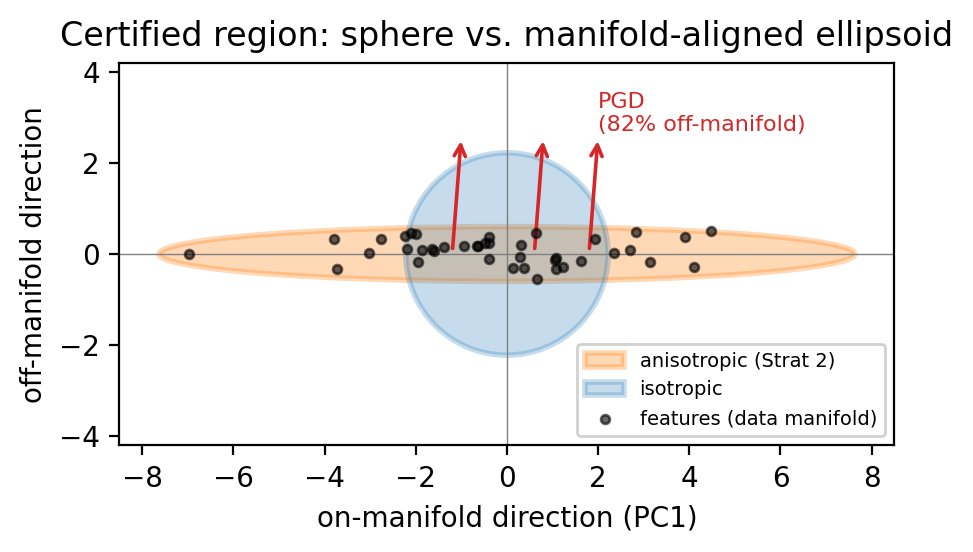
\includegraphics[width=0.92\linewidth]{figures/sphere_vs_ellipsoid.png}
\caption{Isotropic smoothing certifies a sphere (equal in all directions); manifold-aware smoothing certifies an ellipsoid that extends far along the data manifold and little off it. PGD attacks are $82\%$ off-manifold ($\cos^2\theta\!\approx\!0.18$), where the classifier is provably invariant.}
\label{fig:ellipse}
\vspace{-0.3cm}
\end{figure}

\noindent\textbf{Anisotropic smoothing (headline).} Table~\ref{tab:aniso} reports three PCA-aligned strategies at \emph{equalized} budget. Concentrating noise in the decision-relevant subspace (Strategy~2, subspace projection) yields an on-manifold radius of $7.63$, a $3.4\times$ lift over isotropic ($2.22$), and attains $0\%$ abstention --- every correctly classified sample is certified. The near-zero $R_{\ell_2}$ is by design (Fig.~\ref{fig:ellipse}): the certificate is an ellipsoid with long axes in the $80$ on-manifold directions and tiny axes in the $688$ off-manifold directions where the classifier is invariant. A diagnostic confirms the premise: PGD attack directions place only $\cos^2\theta\!\approx\!0.18$ of their energy on-manifold, so $82\%$ of any ambient attack is wasted, exactly the regime Theorem~\ref{thm:scaling} predicts.

\noindent\textbf{Transfer and degradations.} On LAV-DF \cite{cai2022lavdf}, CertAV transfers at $74.6\%$ accuracy and $61.4\%$ certified accuracy at radius $1.0$, indicating useful but imperfect cross-dataset generalization. Common media degradations (social-media re-encoding, H.264 CRF 28, JPEG-75) preserve $>90\%$ certified accuracy at radius $0.5$. Unimodal certificates can have larger numerical radii but protect only one stream.

\section{Conclusion}
\label{sec:conclusion}

CertAV makes certified robustness practical for audio-visual deepfake detection by placing the guarantee at the level of frozen multimodal features. Its central lesson is geometric: the intrinsic dimension of the representation, not the training procedure, governs certifiability (Theorem~\ref{thm:scaling}), which both predicts encoder behavior and motivates manifold-aware anisotropic smoothing for a $3.4\times$ on-manifold gain. The evaluation logic is released as \texttt{av-robustbench}, a reproducible scaffold for attacks, certificates, degradations, and transfer reporting. The main limitations are the feature-space scope of the certificate (our empirical Lipschitz composition is a bridge, not a worst-case input proof), the approximate rather than exact subspace invariance underlying Theorem~\ref{thm:scaling} ($\cos^2\theta\!=\!0.18\!\neq\!0$), single-dataset evaluation, and the cost of Monte Carlo certification.

\bibliographystyle{IEEEbib}
\bibliography{refs}

\end{document}
